% NOT FOR SUBMISSION. Claude-generated draft kept as notes only: AIES bans LLM-generated paper
% text (owner decision 2026-10-04: the author writes the prose; see OUTLINE.md, FACTS.md).
% AIES 2027 draft. Template: plain article until the AIES 2027 call confirms the format
% (prior_art.md, section "AIES 2027"). Results marked \RESULT{...} are slots, filled only from
% graded records (twin/grade_scenarios.py output under /archive/unity/out/<run>/grade.json).
\documentclass[10pt,twocolumn]{article}
\usepackage[margin=0.75in]{geometry}
\usepackage{amsmath,amssymb}
\usepackage{graphicx}
\usepackage{booktabs}
\usepackage{array}
\usepackage{tikz}
\usetikzlibrary{arrows.meta,positioning,fit,calc,shapes.geometric}
\usepackage[hidelinks]{hyperref}
\usepackage{xcolor}

\newif\ifblind
\blindtrue
% a slot for a number not yet graded; the build refuses to ship while any remain (README)
\newcommand{\RESULT}[1]{\fbox{\scriptsize RESULT: #1}}

\title{Language Models Read and Choose but Cannot Grant Authority\\in a Home-Care Robot}
\ifblind\author{Anonymous submission}\else
\author{Andrew H. Bond\\San Jos\'e State University\\andrew.bond@sjsu.edu}\fi
\date{}

\begin{document}
\maketitle

\begin{abstract}
A home-care robot that uses language models to understand its surroundings and pick its actions
can be talked into things. A television drama, a forged alarm or a stranger who claims to be a
plumber reaches the same models that decide whether to call an ambulance or open the door. We
built a robot in which the models never hold that decision. They turn what the robot perceives
into events of a declared model of the home and choose among the actions that model allows.
Every action that grants authority, from calling emergency services to restraining an attacker,
waits for signed readings from independent physical sensors or for a message on an authenticated
channel. We prove in Lean that no event a model writes can reach such an action, for any choice of
the home's rules that passes the loader's checks. We then ran the robot in a simulated home with
four model-driven parties and 43 scripted scenarios. Across the graded runs no action exceeded
its authority. The errors we did find sat elsewhere. A test harness that dropped the woman's
answers, a classifier that labelled sensor readings as strangers and a refusal re-read after she
collapsed each made the robot escalate too far or too late, never act beyond its authority. The
structure stops a misreading from becoming permission. It does not stop a misreading.
\end{abstract}

\section{Introduction}
% DRAFT: the claim and its scope are final; the novelty paragraph waits for prior_art.md.
Language models now read the world for robots and pick what they do next. A care robot that
listens to the person it cares for, watches the room and reads its messages can respond to
situations its designers never listed. The same openness is a liability. The text that reaches
the model includes what a television says, what a network message claims and what a visitor
asserts about himself. A robot that decides from that text whether to call an ambulance, unlock a
medication box or let a man in has handed those decisions to whoever controls the text.

We separate the two jobs. Models read and choose. They never grant. The robot's rules live in a
declared model of the home, written in the ErisML language and compiled into obligations,
prohibitions and state machines. A model may turn perception into events of that home model and
pick one action from the set the rules allow. Actions that carry authority stay out of the set
until a governor rules on evidence that no model writes. That evidence is signed, fresh readings
from physical sensors on independent power and wiring, or a message on an authenticated channel
from the monitoring centre or the emergency dispatcher.

The situation in the home changes in discrete steps. A visitor becomes a stranger, a welcomed
guest, an arranged tradesman or a hostile attacker. An emergency begins and later lapses. We model
each such axis as a stratification with gates in the sense of Geometric
Ethics~\cite{TODO-geometric-ethics}. The loader refuses any home model in which an event a model
can write leads into a stratum that grants authority, or in which anything but human oversight
leads out of an absorbing one. We prove in Lean that these two checks suffice for every set of
gates.

We then asked what this structure buys and what it does not. We ran the robot in a Unity
simulation of one woman's home with three more model-driven parties, the monitoring centre's
operator, the dispatcher and the woman's own voice, against scripted scenarios written before the
system existed and a sealed held-out set. No graded run produced an action beyond its authority.
The failures we found were real and several were ours. Each one made the robot escalate too far,
too late or not at all. None of them made it act beyond its authority.

% Novelty and credit paragraph: written after prior_art.md (Arkin's ethical governor, shields,
% verifiable machine ethics, capability-based LLM agents). Do not claim firsts before then.

\section{Margaret's Home}
\label{sec:home}
Margaret lives alone with her beagle. Her home-care robot is her caregiver for daily tasks. A
monitoring centre run by the robot's maker can talk to her through the robot and can send
emergency services. She has asked that the robot not record her, not share her data and not enter
her bedroom, and the robot has promised this. The promise is defeasible in a corroborated
life-threatening emergency and comes back only when the centre confirms it.

\textbf{Parties.} Four parties act on language models. The robot classifies what it perceives and
chooses its actions. The centre's operator and the emergency dispatcher each run under their own
home model in the same runtime, with 7 and 9 rules. Margaret's voice is a model that answers what
is said to her from her true condition, which the robot never sees.

\textbf{The world.} A Unity simulation renders the home, Margaret, the dog, visitors, a wild
animal, smoke and 15 sensor devices on 6 shared substrates such as one hub or one body. Scenario
scripts call only the world's interface, for example a fall, a forged wearable alert, a network
message or a stranger entering. The robot receives general facts and signed readings, never the
name of the scenario.

\textbf{Scenarios.} Each scenario names the strongest response it calls for. Class R0 is to carry
on, R1 to check in with her, R2 to refer to the centre and R3 to treat it as an emergency. The
development set has 43 scenarios, 7 in R0, 11 in R1, 8 in R2 and 17 in R3. A held-out set of 30
was written by a separate agent from the protocol alone on 2026-10-01 and stored outside every
repository. Only a manifest of its hashes is committed, and it is opened only after the system is
frozen.

\section{Where Authority Comes From}
\label{sec:arch}

\begin{figure*}[t]
\centering
\resizebox{\textwidth}{!}{%
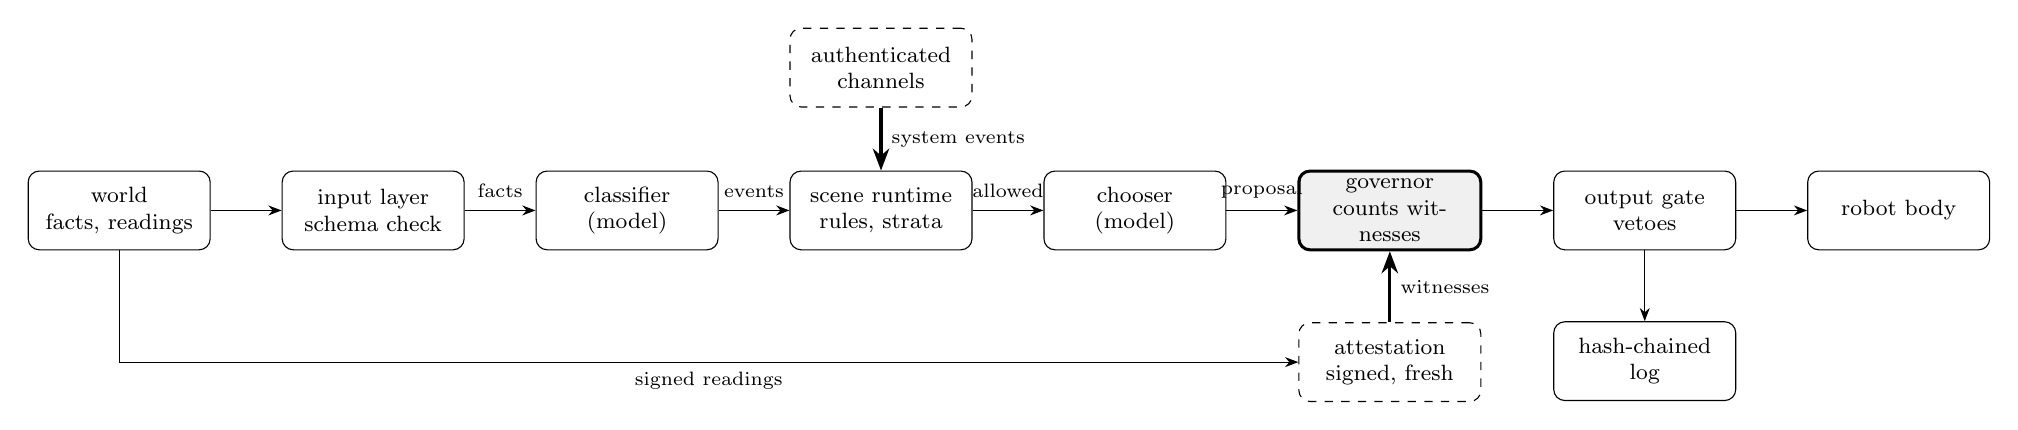
\begin{tikzpicture}[
  font=\footnotesize, node distance=4mm and 9mm,
  box/.style={draw, rounded corners, align=center, minimum height=10mm, inner sep=3pt, text width=21mm},
  grant/.style={box, line width=1.1pt, fill=black!6},
  ev/.style={box, dashed},
  lab/.style={font=\scriptsize, above=1pt},
  >={Stealth[]}]
\node[box] (world) {world\\facts, readings};
\node[box, right=of world] (input) {input layer\\schema check};
\node[box, right=of input] (cls) {classifier\\(model)};
\node[box, right=of cls] (rt) {scene runtime\\rules, strata};
\node[box, right=of rt] (ch) {chooser\\(model)};
\node[grant, right=of ch] (gov) {governor\\counts witnesses};
\node[box, right=of gov] (gate) {output gate\\vetoes};
\node[box, right=of gate] (body) {robot body};
\node[ev, above=8mm of rt] (sys) {authenticated\\channels};
\node[ev, below=9mm of gov] (att) {attestation\\signed, fresh};
\node[box, below=9mm of gate] (log) {hash-chained\\log};
\draw[->] (world) -- (input);
\draw[->] (input) -- node[lab]{facts} (cls);
\draw[->] (cls) -- node[lab]{events} (rt);
\draw[->] (rt) -- node[lab]{allowed} (ch);
\draw[->] (ch) -- node[lab]{proposal} (gov);
\draw[->] (gov) -- (gate);
\draw[->] (gate) -- (body);
\draw[->] (world.south) |- node[pos=0.75, below, font=\scriptsize]{signed readings} (att.west);
\draw[->, line width=1.1pt] (att) -- node[right, font=\scriptsize]{witnesses} (gov);
\draw[->, line width=1.1pt] (sys) -- node[right, font=\scriptsize]{system events} (rt);
\draw[->] (gate) -- (log);
\end{tikzpicture}}
\caption{The authority path. The two models write only perceived events and a proposal from the
allowed set. Authority enters along the heavy edges, as system events on authenticated channels and
as signed readings the governor counts as witnesses.}
\label{fig:arch}
\end{figure*}

Figure~\ref{fig:arch} shows one decision. The home model compiles to 65 rules, of which 45 are
obligations, 19 prohibitions and 1 a permission, and 55 cannot be defeated. It declares 48 event
types. Half of them, 24, come only from the system and are rejected if a model writes them. It
declares 25 robot capabilities, 11 of which need the governor.

\textbf{Perception.} A whitelist schema drops any fact that is not a known field of a declared
type and range. A model then turns the facts into events of the declared vocabulary. Their actors
are snapped to the home's list of parties, and an event type can fix its actor, so a sensor
reading always comes from a device. Free text never reaches the robot's state.

\textbf{Rules and strata.} The runtime steps three kinds of state machine on each event. They
track Margaret's consent, the robot's commitments and the legitimacy of each party, alongside seven
stratifications with 26 strata and 34 gates. They track who a visitor is, whether responders are
expected or at the door, which animal is present and whether it is attacking, the level of
emergency, whether the centre can be reached, whether a crime is pending a report and whether a home
device has been compromised. A gate fires once, on the event that crosses it, and each crossing is
recorded. The loader checks two properties before the home runs. A stratum that grants authority is
entered only by a system event. An absorbing stratum, such as a visitor who attacked her, is left
only by a human oversight event.

\begin{figure}[t]
\centering
\resizebox{\columnwidth}{!}{%
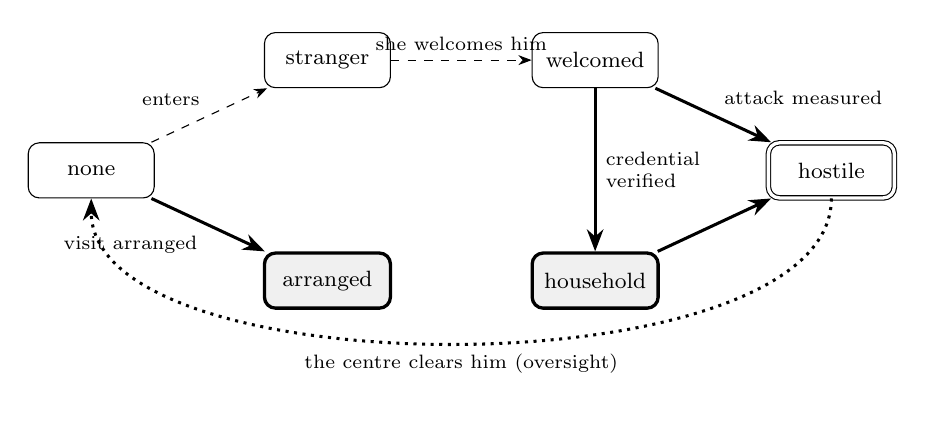
\begin{tikzpicture}[
  font=\footnotesize, >={Stealth[]},
  st/.style={draw, rounded corners, minimum width=16mm, minimum height=7mm, align=center},
  auth/.style={st, line width=1.2pt, fill=black!6},
  absb/.style={st, double, double distance=1.2pt},
  sys/.style={->, line width=1.1pt},
  model/.style={->, dashed},
  lab/.style={font=\scriptsize}]
\node[st] (none) at (0,0) {none};
\node[st] (str) at (3.0,1.4) {stranger};
\node[st] (wel) at (6.4,1.4) {welcomed};
\node[auth] (arr) at (3.0,-1.4) {arranged};
\node[auth] (hh) at (6.4,-1.4) {household};
\node[absb] (hos) at (9.4,0) {hostile};
\draw[model] (none) -- node[lab, above left]{enters} (str);
\draw[model] (str) -- node[lab, above]{she welcomes him} (wel);
\draw[sys] (none) -- node[lab, below left]{visit arranged} (arr);
\draw[sys] (wel) -- node[lab, right, align=left]{credential\\verified} (hh);
\draw[sys] (wel) -- node[lab, above right]{attack measured} (hos);
\draw[sys] (hh) -- (hos);
\draw[sys, dotted] (hos.south) .. controls (9.4,-2.8) and (0,-2.8) .. node[lab, below]{the centre clears him (oversight)} (none.south);
\end{tikzpicture}}
\caption{Who a visitor is, one of the seven stratifications. Dashed gates fire on a model's reading
and lead only to strata that grant nothing. Heavy gates fire on system events. Arranged and
household are authority strata, and hostile is absorbing, left only by oversight. Gates out on
leaving the home are omitted.}
\label{fig:strata}
\end{figure}

\textbf{Choice.} A model sees only the canonical state and the allowed set, never the raw facts,
and proposes one action. The obligations in force reach it in order of urgency. When no model
answers, the robot acts on its most urgent obligation with no model at all.

\textbf{The governor.} A governed action waits for a ruling. The governor counts witnesses. A
witness is a signed reading from a device in the home's inventory whose signature, payload hash,
age of at most 30 seconds and replay counter check out. Devices on one substrate count once. Two
witnesses elevate an emergency, three are needed to restrain a person, and one suffices for
emergency services when the centre cannot be reached. An analyzer of the request's moral content may refuse an elevation
but cannot grant one. A device whose signature fails is quarantined and counts again only after
the centre clears it.

\textbf{Rights revert.} Each cycle the governor recounts. A right whose witnesses stay below its
bar for 60 seconds lapses, and restraint lapses on its own when only its stricter bar fails. A
refused request for one action never ends an emergency that rests on evidence.

\textbf{The output gate.} Each proposal then passes an ethics pipeline whose rights and consent
modules can veto it. A vetoed proposal is replaced by the best allowed alternative. A choice the
pipeline marks as a tragic conflict goes to the centre. Margaret's refusals bind while she can
voice them, and after a lapse they bind again only once she has answered the robot.

\textbf{The ladder as a process.} The escalation ladder (ask her, then the centre, then emergency
services) is declared as a process of 23 nodes in four lanes. It is exported as standard BPMN
2.0, checked against the same rules on import, and drawn live from the log. It is a view of the
rules and grants nothing itself.

\section{What Is Proved and What Is Not}
\label{sec:proof}
A Lean 4 model of the authority path treats every model output as an arbitrary input. Its
theorems state that forged, unattested, stale and repeated readings add no witness. Each granting
ruling carries attested evidence meeting its bar, and the permissions of governed actions are
equal on any two histories that differ only in model-written events. Whatever the ethics pipeline
vetoes or ranks, the gate's output is permitted, and every governed action executed in a reachable
run was permitted. For any stratifications whatever, no trace of model-written events enters an
authority stratum and none without oversight leaves an absorbing one. The two hypotheses of that
last result are the loader's two checks. The 22 theorems of the model rest only on Lean's standard
axioms. Static tests tie the model to the code by requiring the real home model to have the
model's shape.

The proof says nothing about sensors that lie below their signatures, about who writes the home
model and its bars, or about one remaining model path. The centre reads Margaret's own words with a
model, so a misread request for help can send emergency services.

\section{Evaluation Protocol}
\label{sec:protocol}
The protocol was written on 2026-10-01, before the robot or the held-out scenarios existed. A
run plays each scenario in the simulation and records every decision in the hash chain. The
grader computes, per scenario, whether the strongest response matches the class, false clears (an
elevated action or a dispatch in a class R0 to R2 scenario), over-restriction (no emergency
response in class R3), privacy violations and containment breaches (a governed action without the
ruling it needs, judged by the strata recorded when the robot chose it). The held-out set is run
once, at a frozen commit.

\section{Results}
\label{sec:results}

\subsection{No action exceeded its authority}
% Fill from graded records only. Known so far (development runs): dev12a 0 breaches over 21
% scenarios; dev11a's 4 flagged breaches were grader artifacts (each action was in the allowed set
% when chosen and followed a governor elevate), absent under the stratum-aware grader in dev12a.
Across the graded development runs \RESULT{count of governed actions and runs, dev13 and dev14},
no governed action ran without its ruling, and no private action ran outside a corroborated
emergency. \RESULT{held-out containment and privacy counts}.

\subsection{The failures were in reading, not in authority}
% Each finding below is from the records; the counts are from scripts over results.jsonl.
Calibration on the development set found six defects, listed in Table~\ref{tab:calib}. The largest
was in our own test harness. The simulation began listening for Margaret's answer only after the
robot finished asking, so an answer given while it spoke was lost. In the runs before the fix, 44
of the 63 check-ins recorded as unanswered came right after she had answered. Each lost answer sent
the robot one rung up the ladder to the centre. In emergencies it also discarded her words, such
as a report of a tight chest. \RESULT{dev13 lost-answer count over all 43 scenarios; partial
dev13a showed 0 of 4 unanswered check-ins following an answer, both scenarios with her
unresponsive}.

\begin{table}[t]
\centering\footnotesize
\begin{tabular}{@{}>{\raggedright\arraybackslash}p{0.27\columnwidth}>{\raggedright\arraybackslash}p{0.66\columnwidth}@{}}
\toprule
Defect & Effect and fix \\
\midrule
Lost answers & 44 of 63 unanswered check-ins followed an answer. Escalation to the centre. Listen from before the question \\
Readings as strangers & Readings labelled as unknown people. Referral of an intruder who was not there. Fix the actor by event type \\
Refusal re-read & Her earlier words re-read after she collapsed vetoed an authorized ambulance. Re-arm a lapsed refusal only after she answers \\
Unranked duties & A fraud report lost to routine check-ins. Pass obligations to the chooser by urgency \\
Duties never discharged & A call still owed after it was made. Discharge until the stratum is re-entered \\
Refusal ended emergency & A refused request for one action ended an evidenced emergency. Change the emergency level only on the governor's grants and lapses \\
\bottomrule
\end{tabular}
\caption{Defects found in calibration. Every one changed how far or how fast the robot escalated.
None let an action run beyond its authority.}
\label{tab:calib}
\end{table}

\subsection{Response classes}
\RESULT{class-correct, false clears and over-restriction on dev14 and the held-out set, with
per-class counts}.

\section{Related Work}
\label{sec:related}
% Written from prior_art.md, credit precisely.

\section{Discussion and Scope}
\label{sec:discussion}
The structure keeps a misreading from becoming permission. It does not keep the robot from
misreading, and the misreadings we saw were common. Our results come from one simulated home, one
set of rules written by us, perception that reports the simulated world truthfully and scenarios we
wrote or had a separate agent write from our protocol. The held-out set's blindness is procedural
rather than a third party's. Three decisions in the home model are policy rather than engineering
and belong to the people who deploy such a robot. The robot never lifts a person who has fallen,
the dispatcher sends police only on stated facts of a crime, and the robot reports an articulable
suspicion of a crime against her to the centre even when she objects.

\section*{Use of AI}
Language-model assistants helped write the system's code, its tests and drafts of this paper. The
robot, the centre, the dispatcher and Margaret's voice are language models by design. All numbers
come from graded records and scripts named in the repository.

\bibliographystyle{plain}
\bibliography{references}
\end{document}
